\chapter{Конструкторская часть}

\section{Общие сведения}

Положение объектов сцены в пространстве описывается с помощью
мировой системы координат, при этом ось Oz должная быть направлена вверх.

Общий алгоритм работы программы можно описать следующим образом:

\begin{enumerate}
	\item Задать объекты сцены (камера, пол, источник света, слайм);
	\item Для каждого кадра:
	\begin{enumerate}
		\item Если пользователь изменил характеристики объектов сцены, установить новые характеристики объектов;
		\item Если пользователь пытается захватить точку слайма, найти и запомнить ее;
		\item Определить силы, действующие на точки слайма;
		\item Изменить скорости точек слайма в соответствии с действующими на них силами;
		\item Переместить точки слайма, в соответствии с их скоростями;
		\item Если пользователь захватил точку, вернуть ее в исходное положение;
		\item Вывести изображение на экран.
	\end{enumerate}
\end{enumerate}

\section{Разработка структур данных, необходимых для хранения информации о слайме}

Моделируемый объект можно представить в виде множества точек, соединенных между собой пружинами. на рисунке \ref{slime_struct} приведена диаграмма структур данных, необходимых для хранения информации о слайме.

\begin{figure}[H]
	\centering
	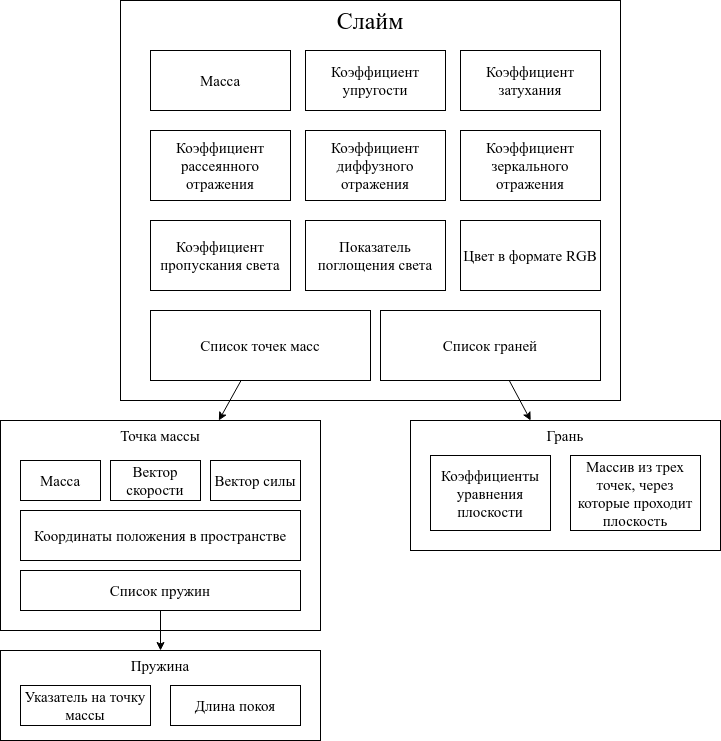
\includegraphics[width=0.8\linewidth]{slime_struct}
	\caption{Структура хранения информации о слайме}
	\label{slime_struct}
\end{figure}

Слайм содержит в себе данные для визуализации и физического моделирования, а также линейные односвязные списки точек масс и граней.

Точка массы описывает элемент поверхности слайма. Данная структура содержит в себе значение массы, вектора скорости и силы для физических расчетов, координаты точки и линейный односвязный список пружин. Сами пружины представляют собой пары, которые содержат в себе указатель на точку массы, с которой есть соединение, и значение длины покоя, при которой сила упругости пружины равна нулю.

Грань нужна для корректной работы реализации алгоритма обратной трассировки. Она содержит в себе коэффициенты уравнения~\eqref{plane_eq} плоскости и массив из трех точек, через которые проходит грань. Ребра, соединяющие эти точки, ограничивают плоскость, и поэтому грань имеет форму треугольника.

\section{Генерация слайма}

Для получения точек масс слайма производится рекурсивное
деление исходных треугольных граней тела на новые треугольники посредством
бисекции, то есть деления сторон треугольников пополам. До разбиения граней
объем представляет собой икосаэдр. Таким образом, поверхность слайма будет представлять собой трехмерную фигуру с треугольными гранями. После разбиения, полученные точки масс соединяются друг с другом пружинами.

Пример разбиения граней приведен на рисунке \ref{split_exmpl}.

\begin{figure}[H]
	\centering
	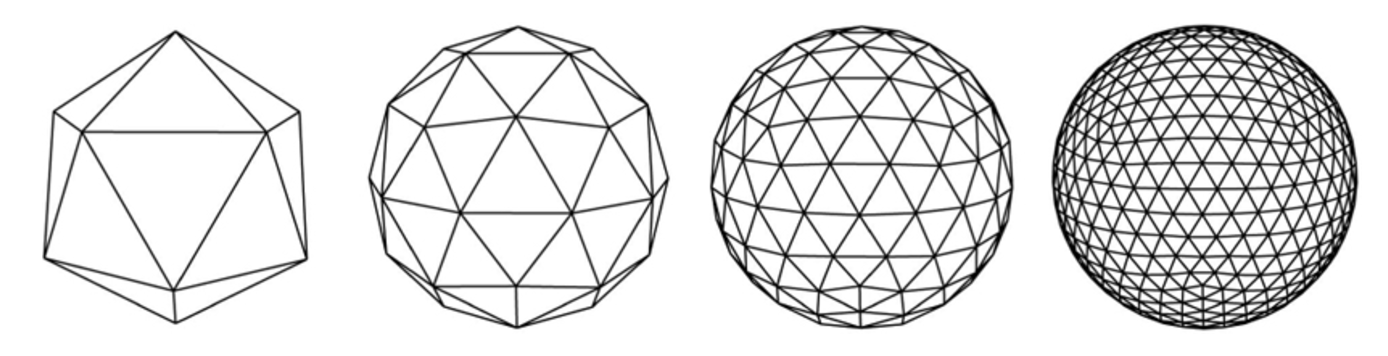
\includegraphics[width=\linewidth]{split_exmpl}
	\caption{Деление граней икосаэдра посредством бисекции}
	\label{split_exmpl}
\end{figure}

\section{Разработка алгоритма расчета физических параметров слайма}

На рисунке \ref{phys} представлена схема алгоритма расчета физических параметров слайма.

\begin{figure}[H]
	\centering
	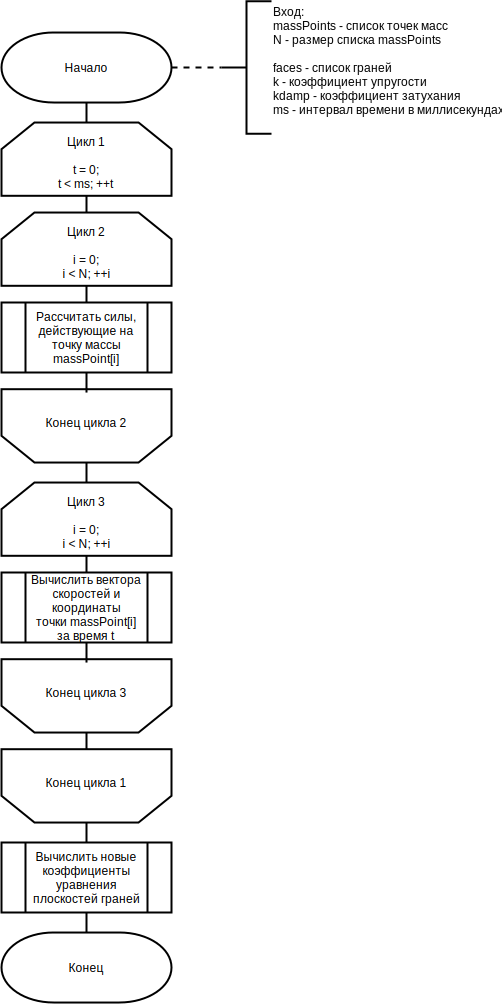
\includegraphics[width=0.6\linewidth]{phys}
	\caption{Схема алгоритма расчета физических параметров слайма}
	\label{phys}
\end{figure}

\subsection{Вычисление векторов сил, действующих на точки масс}

На каждую точку массы действуют три силы:

\begin{itemize}
	\item сила тяжести;
	\item сила упругости со стороны пружины;
	\item сила затухания со стороны демпфера;
\end{itemize}

Вектор силы тяжести вычисляется по формуле:

\begin{equation}\label{mg}
	F_{\text{тяж}_i} = m_i g,
\end{equation}
где $m_i$ - масса $i$-ой точки,\\
\text{~~~~~} $g$ - вектор ускорения свободного падения, $|g| = 9.81 \frac{\text{Н}}{\text{м}}$.

Сила упругости определяется по закону Гука:

\begin{equation}\label{hooke}
	F_{\text{упр}_{ij}} = -k (|x_{ij}| - l_{ij}) \frac{x_{ij}}{|x_{ij}|},
\end{equation}
где $k$ - жесткость пружины, соединяющей точки масс $i$ и $j$;\\
\text{~~~~~}$x_{ij}$ - разница радиус-векторов точек масс $j$ и $i$ соответственно,\\
\text{~~~~~}$l_{ij}$ - расстояние между точками масс $i$ и $j$, при котором сила упругости равна нулю.

Затухающая сила вычсляется по формуле:

\begin{equation}\label{damp}
	F_{\text{сопр}_{ij}} = -k_d \frac{(v_{ij}; x_{ij})}{(x_{ij}; x_{ij})} \frac{x_{ij}}{|x_{ij}|},
\end{equation}
где $k_d$ - коэффициент затухания,\\
\text{~~~~~}$x_{ij}$ - разница радиус-векторов точек масс $j$ и $i$ соответственно,\\
\text{~~~~~}$v_{ij}$ - разница векторов скокростей точек масс $j$ и $i$ соответственно.

В итоге, используя формулы \eqref{mg}, \eqref{hooke} и \eqref{damp}, можно вычислить равнодействующую всех сил, приложенных к $i$-ой точку массы:

\begin{equation}\label{f}
	F_i = F_{\text{тяж}_i} + \sum_{j}^{M} (F_{\text{упр}_{ij}} + F_{\text{сопр}_{ij}}),
\end{equation}
где $M$ - количество пружин, которые имеет $i$-ая точка массы.

\subsection{Вычисление новых координат точек масс}

Вектор ускорения точки вычисляется по второму закону Ньютона:

\begin{equation}\label{sln}
	a_i = \frac{F_i}{m_i},
\end{equation}
где $m_i$ - масса $i$-ой точки,\\
\text{~~~~~}$F_i$ - равнодействующая всех сил, приложенных к $i$-ой точку.

В соответствии с полученным ускорением, вычисляется вектор скорости $i$-ой точки массы по формуле:

\begin{equation}\label{velocity}
	v_i = v_{0_i} + a_i t,
\end{equation}
где $v_{0_i}$ - начальная скорость $i$-ой точки,\\
\text{~~~~~}$t$ - время, в течении которого изменяется скорость под действием сил, $t = 1~\text{мс}$.

Новые координаты точки вычисляются по формуле:

\begin{equation}\label{new_pos}
	P_i(x, y, z) = P_{0_i}(x_0, y_0, z_0) + v_{0_i} t + a_i t^2,
\end{equation}
где $P_{0_i}(x_0, y_0, z_0)$ - радиус-вектор начального положения $i$-ой точки в пространстве,\\
\text{~~~~~}$v_{0_i}$ - начальная скорость $i$-ой точки,\\
\text{~~~~~}$a_i$ - ускорение $i$-ой точки,\\
\text{~~~~~}$t$ - время, в течении которого изменяется скорость под действием сил, $t = 1~\text{мс}$.

\section{Разработка алгоритма обратной трассировки лучей}

На рисунке \ref{ray_tracing} приведена схема алгоритма обратной трассировки лучей.

\begin{figure}[H]
	\centering
	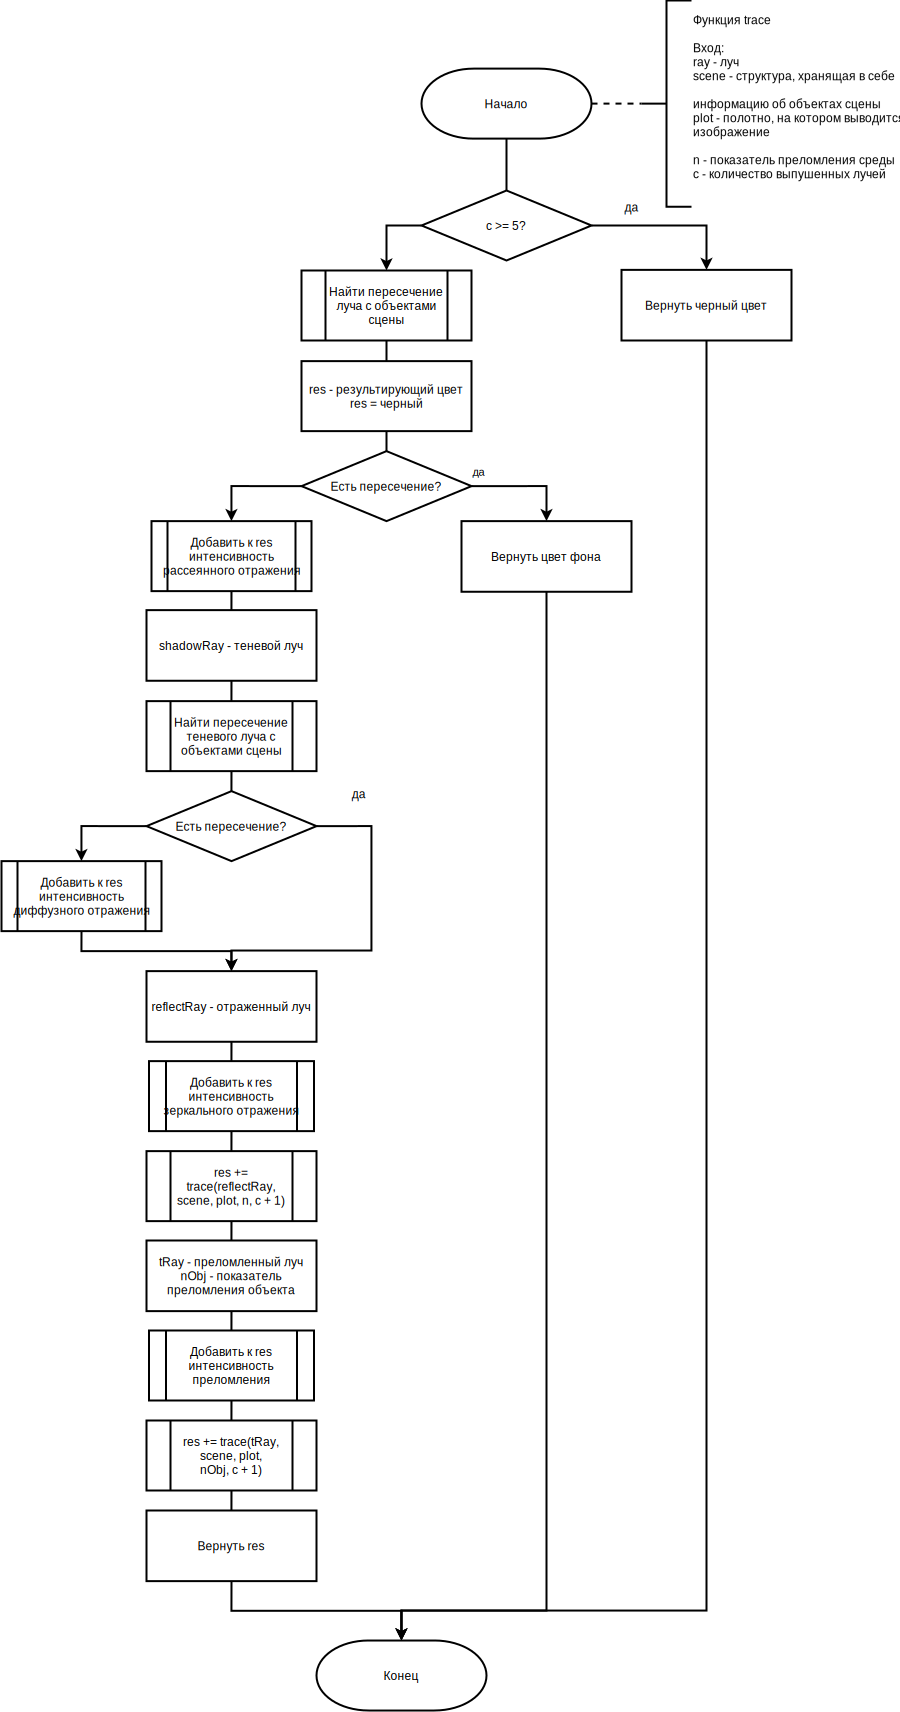
\includegraphics[width=0.8\columnwidth]{ray_tracing}
	\caption{Схема алгоритма обратной трассировки лучей}
	\label{ray_tracing}
\end{figure}

\section{Захват точки слайма пользователем}

Программа моделирования слайма должна обеспечивать управление объектом. В частности, пользователь должен иметь возможность растягивать и вдавливать тело.

На рисунке \ref{grabbing} приведена схема алгоритма захвата точки слайма пользователем.

\begin{figure}[H]
	\centering
	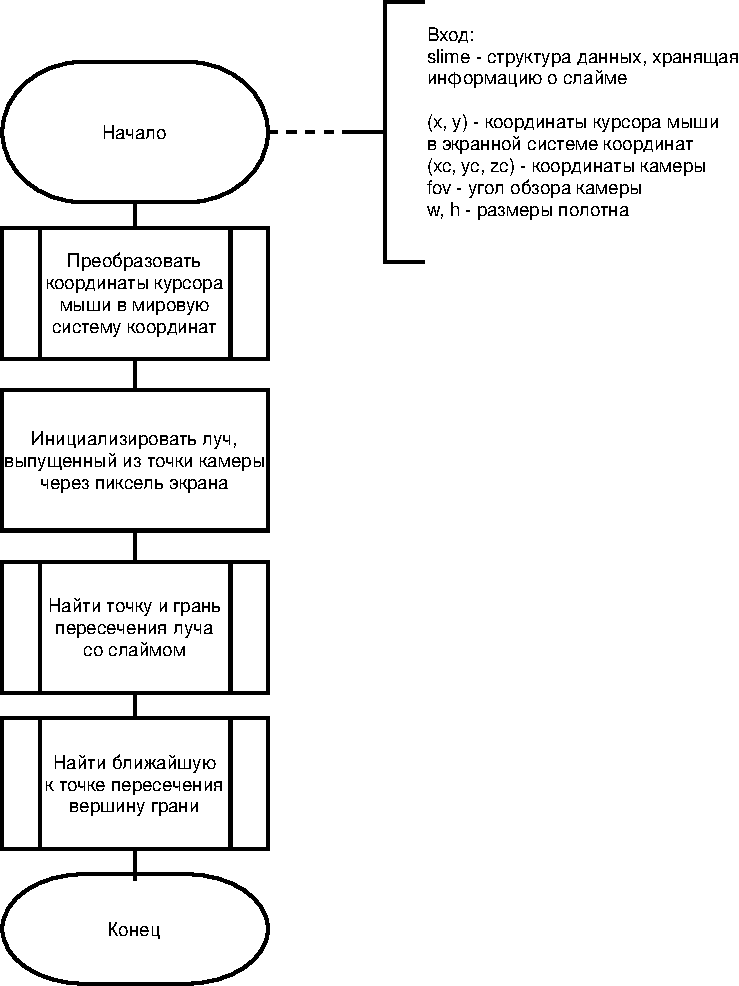
\includegraphics[width=0.6\linewidth]{grabbing}
	\caption{Схема алгоритма захвата точки слайма пользователем}
	\label{grabbing}
\end{figure}

\section*{Вывод}
В данном разделе были разработаны алгоритмы, необходимые для разработки программного обеспечения.

\clearpage
